%%%%%%%%%%%%%%%%%%%%%%%%%%%%%%%%%%%%%%%%%%%%%%%%%%%%%%%%%%%%%%%%%%%%%%
\chapter{Related Work}
\label{ch:RelatedWork}

In this chapter we are presenting a couple of related publications, this work can be referenced to. The sections are oriented on the task and problems mentioned in \autoref{sec:Introduction:goals}.


\section{Application Monitoring}
\label{sec:RelatedWork:appl_mon}

The monitoring of software systems is common task in many research fields. Automated data-flow analysis, software profiling and hardware utilization are only a small selection of groups, using this term. In the following, we use application monitoring in the sense of online extraction of runtime data form a (distributed cloud) application for architecture optimization.

R-PRIS (\autoref{sec:RelatedWork:privacyanalysis}) and Kieker are application monitoring frameworks. While iObserve uses Kieker to extract the desired information, R-PRIS is independent from other programs. Neither of them uses a meaningful architecture description language (ADL) to process and store the gathered information. iObserve however gathers the transmitted data, processes them and stores them into a PCM model, enabling all kind of PCM-based applications to use the gathered information.
\todo{gather more details \& Refs} 


\section{Privacy Analysis}
\label{sec:RelatedWork:privacyanalysis}

R-PRIS is a monitoring and analysing tool for distributed cloud systems. Like iObserve, R-PRIS updates a runtime model by monitoring the cloud systems. During the analysis phase the model is checked for (potential) privacy violations.

Like Kieker, R-PRIS combines push-based heartbeat monitoring with event processing, and graph grammars for efficiently updating those models \cite{Schmieders.}. R-PRIS uses a formal specification for geo-location policies. These consists of data classification $S$, data content types $T$ and geo-locations $L$. Every specified policy $p = (S, T, L)$ is forbidden. This means, a data modelling is required with a \textit{Classification} and the containing \textit{ContentType} (see \autoref{fig:rpris_metamodel}). During privacy analysis R-PRIS checks whether a privacy protected information can be accessed from an non-privacy compliant location. This can be transformed into an st-connectivity problem, a standard problem in graph theory and analysis. Based on the runtime model (\autoref{fig:rpris_model}) - with its meta-model (\autoref{fig:rpris_metamodel}) - R-PRIS performs a reachability check \cite{Schmieders.2015}. 

\begin{figure}[h]
	\centering
	\begin{minipage}[b]{0.48\textwidth}		
		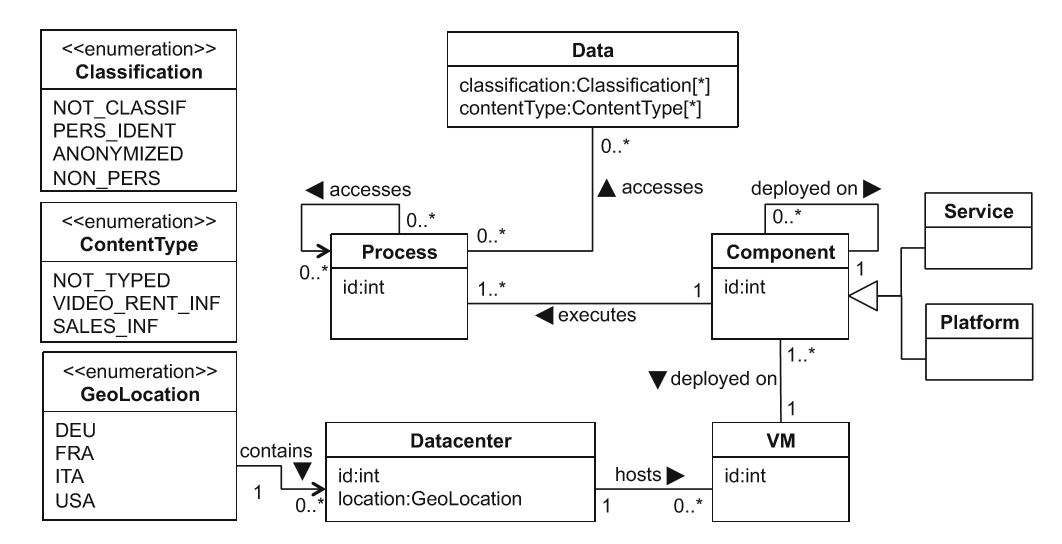
\includegraphics[width=\textwidth]{pictures/rpris_metamodel.jpg}
		\caption{R-PRIS meta-model}
		\label{fig:rpris_metamodel}
	\end{minipage}
	\begin{minipage}[b]{0.48\textwidth}
		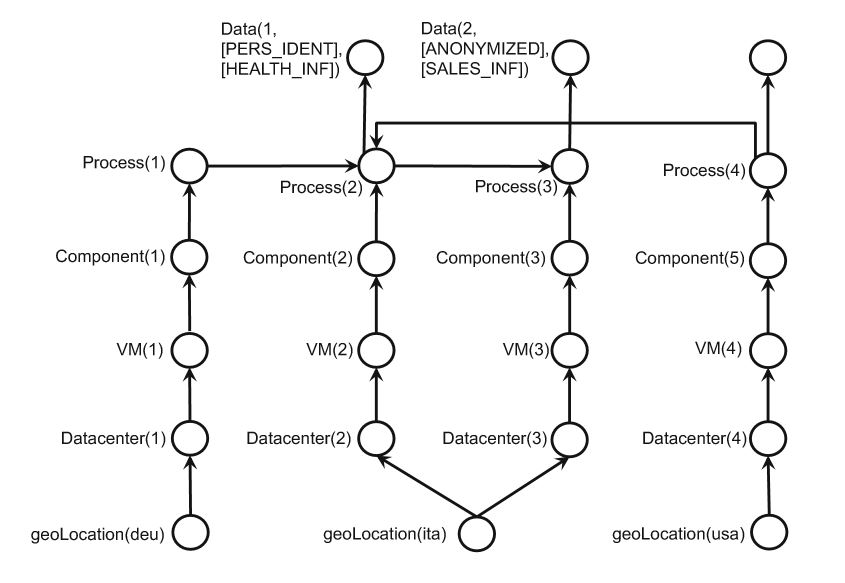
\includegraphics[width=\textwidth]{pictures/rpris_model.jpg}
		\caption{R-PRIS runtime model}
		\label{fig:rpris_model}
	\end{minipage}
\end{figure}

In terms of software, R-PRIS searches for communication paths in the distributed system, which can potentially transmit personal data to a non-privacy compliant geo-location. In order to detect these communication paths a policy $p$ must be specified, representing exactly this case, which however doesn't necessarily communicate private data. As a result, a lot of policies have to be specified, which prohibit many potentially harmless communication paths.

Based on their runtime model, Schmieders et al. identified four relevant migration-cases and extracted six required informations to detect a policy violation\cite{Schmieders.2015}:

\begin{table}[h]
	\centering
	\begin{tabular}{r | l}
		\hline
		\textbf{\#} & \textbf{Required information to carry out runtime check}\\
		\hline
		R1 & Interactions of two components\\
		R2 & Access of components to locally stored files\\
		R3 & Meta-information of stored or processed data\\
		R4 & Information on component deployments on physical resources \\
		R5 & Geo-location information of physical resources\\
		R6 & Explicit or implicit information on transitive data transfers\\
		\hline
	\end{tabular}
	\caption{R-PRIS information for runtime privacy checks \cite{Schmieders.2015}}
	\label{tab:rpris_information}
\end{table}


Due to the comparable core task of detecting privacy violations, we are comparing the R-PRIS privacy analysis against the iObserve Privacy privacy analysis. More detailed information on R-PRIS can be found in \cite{Schmieders.}\cite{Schmieders.2015}.

\begin{description}
	\item[Runtime Model] R-PRIS uses the specially developed model shown in \autoref{fig:rpris_metamodel}. Even while it models components, VMs and process, it does not capture the systems architecture as the Palladio Component Model does. Further, it is not known, whether tool support or other compatible programs exist, like the PCM has. 
\end{description}

\begin{description}
	\item[Categorization] We are utilizing a component communication classification, which leads to a component classification and a deployment analysis. Therefore, we do not know what data are actually processed in a component or on a server. R-PRIS, however, tags the data itself, traces the transitive access and prohibits rule violating access. As a result, R-PRIS, uses the more accurate \textit{data tracking}, which requires more information then and a deep knowledge about the observed system then iObserve privacy. While iObserve privacy uses data categorization by hand, the R-PRIS approach does not explain their modelling and categorization process.
\end{description}

\begin{description}
	\item[Rule Compliance] iObserve Privacy is clearly build to stay EU General Data Protection Regulation and HIPAA compliant. Therefore, a simple file input with \textit{save} geo-locations is sufficient. R-PRIS requires a rule input, which specifies prohibited data access. Compared to iObserve privacy, this is a more powerful and flexible input. Nevertheless, it complicates the usage and scales poorly with the system size, deployment locations and data variety, since every prohibited access needs to be specified for every data type per geo-location and content type.
\end{description}



\section{Data-flow Analysis \& Rights Management}
\label{sec:RelatedWork:dataflow}

(Access) Rights Management, like the Bell-LaPadula Model or Role-based access control, are fundamentals in our modern information society. These systems restrict or allow access on certain entities with the intention of information protection. The fundamentals are well researched, so research currently is focused on resource and time efficient rights management in large scale systems like companies, as well as automated rights management on small, mobile devices \cite{Dinger.2008}.

Data-flow Analysis is a hot research topic due to the omnipresence of cloud services and mobile devices with rich data sources. Applications like \textit{JOANA} \cite{Snelting.2014}, \textit{TaintDroid} \cite{Enck.2014}, \textit{Privacy Oracle}  \cite{Jung.2008} or \textit{automated privacy instrumentation} \cite{Suh.2004} are only some of many applications and approaches around data-tracking, data-flow analysis and leak detection. However, nearly all of these approaches are using actual code or information rich models.

For our purposes we need automated data-flow analysis on architecture level, to determine if a system violates privacy regulations. This research is still in its early stages and therefore not suited for applications with our designated level of complexity.


\section{Privacy Analysis}
\label{sec:RelatedWork:privacy_check}

Most research in this field focuses on prevention of policy violation. “However, changes of data geo-locations imposed by migration or replication of the component storing the data are not considered. Data transfers between the client services and further services are not covered. Transitive data transfers that may lead to policy violations thus remain undetected.”\cite{Schmieders.2015}

As mentioned in \autoref{sec:RelatedWork:privacyanalysis}, R-PRIS is searching for potential access violations in the application model, by using a st-connectivity analysis.\cite{Schmieders.2015}\cite{Schmieders.} This approach is overestimating the privacy aspects by not including which kind of data are actually communicated between components and geo-locations. This makes it impractical for many business applications, due to the high likelihood of allowing only deployments on save-considered geo-locations.


\section{Automated Model Optimization \& Modification}
\label{sec:RelatedWork:auto_model_opt}

The research field of model analysis based performance optimizer can be roughly divided into two sections. First, the rule-based approaches, which apply a predefined rule, based on the detected problem, onto the system model. Second, metaheuristic-based approaches, which use a generic framework and evolutionary algorithms for multiple arbitrary quality criteria.\cite{Martens.2010}

PerOpteryx (\autoref{sec:Foundations:peropteryx}) is a metaheuristic-based approach. However, PerOpteryx does not consider a hosts geo-location during its optimization process. This can be changed by adding an allocation constraint, preventing privacy violating deployments. 



\section{Automated Cloud Migration \& Adaptation}
\label{sec:RelatedWork:cloud_migration}

Since the start of cloud computing there has been plenty of research on how to migrate regular on premise applications and software into the cloud. Either software is cloud-enabled in the most automatic fashion possible or the software is cloud-native, meaning specially developed or redesigned, by developers, for running inside the cloud. While there has been good progress semi-automatically cloud-enabled software, the field of migrating cloud applications form one cloud provider to another is just beginning. One of the main issues is resulting in provider individual Cloud-APIs. Current, state of the art is the "Docker" or container-technology, which wraps the application like a VM and is suitable for many cloud provider. Nevertheless, many cloud provider offer special purpose solutions, where a docker solution is not viable. The technology side of cloud to cloud migration will be left out in this thesis. \cite{Jambunathan.February2016}\cite{Binz.2014} 